\documentclass[12pt]{article}

\usepackage{amsmath,amsthm,amsfonts,amssymb,amsxtra}
\usepackage{tikz,array}
\usetikzlibrary{arrows}
\renewcommand{\theenumi}{(\alph{enumi})} 
\renewcommand{\labelenumi}{\theenumi}

\pagestyle{empty}
\setlength{\textwidth}{7in}
\setlength{\oddsidemargin}{-0.5in}
\setlength{\topmargin}{-1.0in}
\setlength{\textheight}{9.5in}

\theoremstyle{definition}
\newtheorem{problem}{Problem}

\begin{document}

\noindent{\large\bf MATH 242}\hfill{\large\bf Test \#3}\hfill{\large\bf
  Summer 2017}\hfill{\large\bf Page 1/5}\hrule

\bigskip
\begin{center}
  \begin{tabular}{|ll|}
    \hline & \cr
    {\bf Name: } & \makebox[12cm]{\hrulefill}\cr & \cr
    {\bf VIP ID:} & \makebox[12cm]{\hrulefill}\cr & \cr
    \hline
  \end{tabular}
\end{center}
\begin{itemize}
\item Write your name and your VIP ID in the space provided above.
\item The test has five (5) pages, including this one and the table of
  Laplace transforms at the end.
\item Show sufficient work to justify all answers unless otherwise
  stated in the problem.  Correct answers with inconsistent work may
  not be given credit. 
\item Credit for each problem is given at the right of each problem
  number. 
\end{itemize}
\hrule

\begin{center}
  \begin{tabular}{|c|c|c|}
    \hline
    &&\cr
    {\large\bf Page} & {\large\bf Max} & {\large\bf Points} \cr
    &&\cr
    \hline
    &&\cr
    {\Large 2} & \Large 60 & \cr
    &&\cr
    \hline
    &&\cr
    {\Large 3} & \Large 20 & \cr
    &&\cr
    \hline
    &&\cr
    {\Large 4} & \Large 20 & \cr
    &&\cr
    \hline\hline
    &&\cr
    {\large\bf Total} & \Large 100 & \cr
    &&\cr
    \hline
  \end{tabular}
\end{center}
\newpage

%%%%%%%%%%%%%%%%%%%%%%%%%%%%%%%%%%%%% Page 2
\noindent{\large\bf MATH 242}\hfill{\large\bf Test \#3}\hfill{\large\bf Summer 2017}\hfill{\large\bf Page 2/5}\hrule

\bigskip
\begin{problem}[60 pts---10 pts each]
Find the Laplace transform of the following functions:
\begin{enumerate}
  \item $f(x) = 3x^2-4x+7$
  \begin{flushright}
  \begin{tikzpicture}
  \draw (-0.75cm, 0.5cm) node{$F(s) =$};
  \draw (0cm,-0.2cm) rectangle (5cm,1.2cm);
  \draw (4cm, 0cm) node {$(s> \quad)$};
  \end{tikzpicture}
  \end{flushright}
  \item $f(x) = x^3 - x^{3/2}$
  \begin{flushright}
  \begin{tikzpicture}
  \draw (-0.75cm, 0.5cm) node{$F(s) =$};
  \draw (0cm,-0.2cm) rectangle (5cm,1.2cm);
  \draw (4cm, 0cm) node {$(s> \quad)$};
  \end{tikzpicture}
  \end{flushright} 
  \item $f(x) = 2e^{3x} - 8e^{-7x} + \cos(\pi x)$
  \begin{flushright}
  \begin{tikzpicture}
  \draw (-0.75cm, 0.5cm) node{$F(s) =$};
  \draw (0cm,-0.2cm) rectangle (5cm,1.2cm);
  \draw (4cm, 0cm) node {$(s> \quad)$};
  \end{tikzpicture}
  \end{flushright}
  \item $f(x) = 3x^2\sin (5x)$
  \vspace{2cm}
  \begin{flushright}
  \begin{tikzpicture}
  \draw (-0.75cm, 0.5cm) node{$F(s) =$};
  \draw (0cm,-0.2cm) rectangle (5cm,1.2cm);
  \draw (4cm, 0cm) node {$(s> \quad)$};
  \end{tikzpicture}
  \end{flushright}
  \item $f(x) = 6xe^{-x}\sin x$
  \vspace{3cm}
  \begin{flushright}
  \begin{tikzpicture}
  \draw (-0.75cm, 0.5cm) node{$F(s) =$};
  \draw (0cm,-0.2cm) rectangle (5cm,1.2cm);
  \draw (4cm, 0cm) node {$(s> \quad)$};
  \end{tikzpicture}
  \end{flushright}
  \item $f(x) = \sin x \cos x$
  \vspace{1cm}
  \begin{flushright}
  \begin{tikzpicture}
  \draw (-0.75cm, 0.5cm) node{$F(s) =$};
  \draw (0cm,-0.2cm) rectangle (5cm,1.2cm);
  \draw (4cm, 0cm) node {$(s> \quad)$};
  \end{tikzpicture}
  \end{flushright} 
\end{enumerate}
\end{problem}


\newpage
%%%%%%%%%%%%%%%%%%%%%%%%%%%%%%%%%%%%% Page 3
\noindent{\large\bf MATH 242}\hfill{\large\bf Test \#3}\hfill{\large\bf
  Summer 2017}\hfill{\large\bf Page 3/5}\hrule

\bigskip
\begin{problem}[20 pts---10 pts each]
Find the inverse Laplace transform of the following functions in the given domains.
\begin{enumerate}
  \item $F(s) = \dfrac{2s-3}{s^2-2s-15}$, $(s>5)$
  \vspace{8cm}
  \begin{flushright}
  \begin{tikzpicture}
  \draw (-0.75cm, 0.5cm) node{$f(x) =$};
  \draw (0cm,-0.2cm) rectangle (5cm,1.2cm);
  \end{tikzpicture}
  \end{flushright} 
  \item $F(s) =\dfrac{s-3}{(s-3)^2+16}$, $(s>3)$
  \vspace{8cm}
  \begin{flushright}
  \begin{tikzpicture}
  \draw (-0.75cm, 0.5cm) node{$f(x) =$};
  \draw (0cm,-0.2cm) rectangle (5cm,1.2cm);
  \end{tikzpicture}
  \end{flushright} 
\end{enumerate}
\end{problem}
\newpage

%%%%%%%%%%%%%%%%%%%%%%%%%%%%%%%%%%%%% Page 4
\noindent{\large\bf MATH 242}\hfill{\large\bf Test \#3}\hfill{\large\bf
  Summer 2017}\hfill{\large\bf Page 4/5}\hrule

\bigskip
\begin{problem}[20 pts]
Use techniques based on the Laplace transform to solve the initial value problem $y''+3y'+2y=x$ that satisfies $y(0)=0, y'(0)=2$.
\vspace{20cm}
\begin{flushright}
  \begin{tikzpicture}
    \draw (0cm,-0.2cm) rectangle (5cm,1.2cm);
  \end{tikzpicture}
\end{flushright}
\end{problem}
\newpage

%%%%%%%%%%%%%%%%%%%%%%%%%%%%%%%%%%%%% Page 5
\noindent{\large\bf MATH 242}\hfill{\large\bf Test \#3}\hfill{\large\bf
  Summer 2017}\hfill{\large\bf Page 5/5}\hrule

\bigskip
\begin{center}
%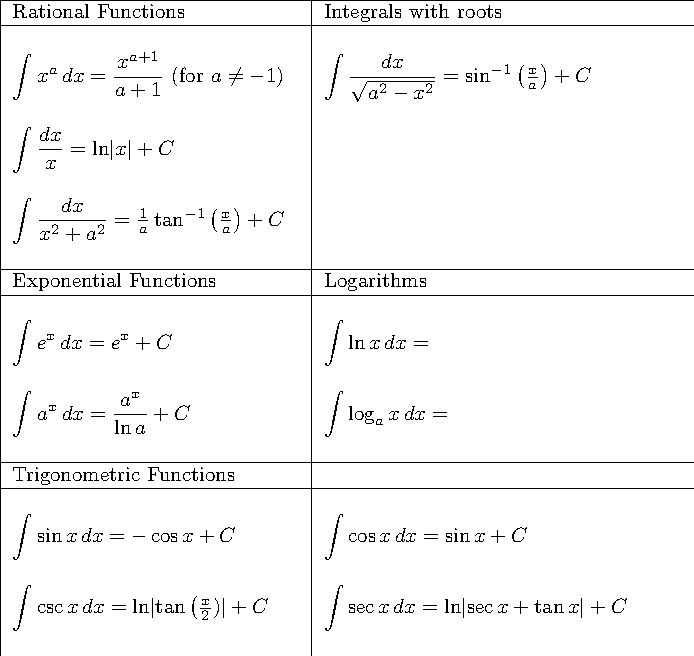
\includegraphics[width=\linewidth]{table.pdf}
\begin{tikzpicture}
  \node[scale=0.97]{
 \begin{tabular}{|m{1.2cm}|m{4.3cm}l||m{2.1cm}|m{4.3cm}l|}
 \hline
    $f(x)$\raisebox{0.5cm} & $\mathcal{L}\{f\}=\int_0^\infty e^{-sx}f(x)\, dx$\raisebox{0.5cm} & &
    \raisebox{0.5cm} & \raisebox{0.5cm} & \\[0.4cm] 
    \hline \hline
    $1$ & $\dfrac{1}{s}$\raisebox{0.6cm} & $s>0$ &
    $cf(x)\pm g(x)$ & $cF(s) \pm G(s)$\raisebox{0.4cm} & $s>max(a,b)$ \\[0.4cm]
    \hline
    $x^n$ & $\dfrac{n!}{s^{n+1}}$\raisebox{0.6cm} & $s>0$ & $e^{\alpha x}f(x)$ & $F(s-\alpha)$\raisebox{0.4cm} & $s>a+\alpha$ \\[0.4cm]
    \hline
    $x^p$ & $\frac{p}{s} \mathcal{L}\{ x^{p-1} \}$\raisebox{0.6cm} & $s>0$ &
    $x^n f(x)$ & $(-1)^n F^{(n)}(s)$\raisebox{0.4cm} & $s>a$ \\[0.4cm]
    \hline
    $e^{\alpha x}$ & $\dfrac{1}{s-\alpha}$\raisebox{0.6cm} & $s>\alpha$ & $f'(x)$ & $s F(s) -f(0)$\raisebox{0.4cm} & $s>a$ \\[0.4cm]
    \hline
    $\sin \beta x$ & $\dfrac{\beta}{s^2+\beta^2}$\raisebox{0.6cm} & $s>0$  &\raisebox{0.4cm} & & \\[0.4cm]
    \hline
    $\cos \beta x$ & $\dfrac{s}{s^2+\beta^2}$\raisebox{0.6cm} & $s>0$ & \raisebox{0.4cm} & & \\[0.4cm]
    \hline
    \end{tabular} };
    \end{tikzpicture}
\end{center}
 
\hrule

\bigskip
\noindent You may use this as scratch paper.  Do not detach from the rest of the test


\end{document}
